%%
%% This is file `acmsmall-submission.tex',
%% generated with the docstrip utility.
%%
%% The original source files were:
%%
%% samples.dtx  (with options: `all,acmsmall,submission')
%% 
%% IMPORTANT NOTICE:
%% 
%% For the copyright see the source file.
%% 
%% Any modified versions of this file must be renamed
%% with new filenames distinct from acmsmall-submission.tex.
%% 
%% For distribution of the original source see the terms
%% for copying and modification in the file samples.dtx.
%% 
%% This generated file may be distributed as long as the
%% original source files, as listed above, are part of the
%% same distribution. (The sources need not necessarily be
%% in the same archive or directory.)
%%
%%
%% Commands for TeXCount
%TC:macro \cite [option:text,text]
%TC:macro \citep [option:text,text]
%TC:macro \citet [option:text,text]
%TC:envir table 0 1
%TC:envir table* 0 1
%TC:envir tabular [ignore] word
%TC:envir displaymath 0 word
%TC:envir math 0 word
%TC:envir comment 0 0
%%
%% The first command in your LaTeX source must be the \documentclass
%% command.
%%
%% For submission and review of your manuscript please change the
%% command to \documentclass[manuscript, screen, review]{acmart}.
%%
%% When submitting camera ready or to TAPS, please change the command
%% to \documentclass[sigconf]{acmart} or whichever template is required
%% for your publication.
%%
%%
\documentclass[manuscript, screen, review]{acmart}
\microtypesetup{expansion=false}
%%
%% \BibTeX command to typeset BibTeX logo in the docs
\AtBeginDocument{%
  \providecommand\BibTeX{{%
    Bib\TeX}}}
\newcommand{\delete}[1]{}
%% Rights management information.  This information is sent to you
%% when you complete the rights form.  These commands have SAMPLE
%% values in them; it is your responsibility as an author to replace
%% the commands and values with those provided to you when you
%% complete the rights form.
\delete{
\setcopyright{acmlicensed}
\copyrightyear{2018}
\acmYear{2018}
\acmDOI{XXXXXXX.XXXXXXX}

%% These commands are for a JOURNAL article.
\acmJournal{JACM}
\acmVolume{37}
\acmNumber{4}
\acmArticle{111}
\acmMonth{8}
 }

%%
%% Submission ID.
%% Use this when submitting an article to a sponsored event. You'll
%% receive a unique submission ID from the organizers
%% of the event, and this ID should be used as the parameter to this command.
%%\acmSubmissionID{123-A56-BU3}

%%
%% For managing citations, it is recommended to use bibliography
%% files in BibTeX format.
%%
%% You can then either use BibTeX with the ACM-Reference-Format style,
%% or BibLaTeX with the acmnumeric or acmauthoryear sytles, that include
%% support for advanced citation of software artefact from the
%% biblatex-software package, also separately available on CTAN.
%%
%% Look at the sample-*-biblatex.tex files for templates showcasing
%% the biblatex styles.
%%
%%
%% The majority of ACM publications use numbered citations and
%% references.  The command \citestyle{authoryear} switches to the
%% "author year" style.
%%
%% If you are preparing content for an event
%% sponsored by ACM SIGGRAPH, you must use the "author year" style of
%% citations and references.
%% Uncommenting
%% the next command will enable that style.
%%\citestyle{acmauthoryear}


%%
%% end of the preamble, start of the body of the document source.
\begin{document}

%%
%% The "title" command has an optional parameter,
%% allowing the author to define a "short title" to be used in page headers.
\title{Automated Construction of Embedded Software IP from Legacy Code: Entity Extraction, Interface Refinement, and Multi-Level Specification Verification}

%%
%% The "author" command and its associated commands are used to define
%% the authors and their affiliations.
%% Of note is the shared affiliation of the first two authors, and the
%% "authornote" and "authornotemark" commands
%% used to denote shared contribution to the research.
\delete{
\author{Ben Trovato}
\authornote{Both authors contributed equally to this research.}
\email{trovato@corporation.com}
\orcid{1234-5678-9012}
\author{G.K.M. Tobin}
\correspondingauthor
\authornotemark[1]
\email{webmaster@marysville-ohio.com}
\affiliation{%
  \institution{Institute for Clarity in Documentation}
  \city{Dublin}
  \state{Ohio}
  \country{USA}
}

\author{Lars Th{\o}rv{\"a}ld}
\affiliation{%
  \institution{The Th{\o}rv{\"a}ld Group}
  \city{Hekla}
  \country{Iceland}}
\email{larst@affiliation.org}

\author{Valerie B\'eranger}
\affiliation{%
  \institution{Inria Paris-Rocquencourt}
  \city{Rocquencourt}
  \country{France}
}

\author{Aparna Patel}
\affiliation{%
 \institution{Rajiv Gandhi University}
 \city{Doimukh}
 \state{Arunachal Pradesh}
 \country{India}}

\author{Huifen Chan}
\affiliation{%
  \institution{Tsinghua University}
  \city{Haidian Qu}
  \state{Beijing Shi}
  \country{China}}

\author{Charles Palmer}
\affiliation{%
  \institution{Palmer Research Laboratories}
  \city{San Antonio}
  \state{Texas}
  \country{USA}}
\email{cpalmer@prl.com}

\author{John Smith}
\affiliation{%
  \institution{The Th{\o}rv{\"a}ld Group}
  \city{Hekla}
  \country{Iceland}}
\email{jsmith@affiliation.org}

\author{Julius P. Kumquat}
\correspondingauthor
\affiliation{%
  \institution{The Kumquat Consortium}
  \city{New York}
  \country{USA}}
\email{jpkumquat@consortium.net}


%%
%% By default, the full list of authors will be used in the page
%% headers. Often, this list is too long, and will overlap
%% other information printed in the page headers. This command allows
%% the author to define a more concise list
%% of authors' names for this purpose.
\renewcommand{\shortauthors}{Trovato et al.}
}
%%
%% The abstract is a short summary of the work to be presented in the
%% article.
\begin{abstract}
   
\end{abstract}

%%
%% The code below is generated by the tool at http://dl.acm.org/ccs.cfm.
%% Please copy and paste the code instead of the example below.
%%
\begin{CCSXML}
<ccs2012>
   <concept>
       <concept_id>10011007.10011074.10011075.10011077</concept_id>
       <concept_desc>Software and its engineering~Software design engineering</concept_desc>
       <concept_significance>500</concept_significance>
       </concept>
   <concept>
       <concept_id>10011007.10011074.10011092.10011096</concept_id>
       <concept_desc>Software and its engineering~Reusability</concept_desc>
       <concept_significance>300</concept_significance>
       </concept>
   <concept>
       <concept_id>10011007.10011074.10011099.10011692</concept_id>
       <concept_desc>Software and its engineering~Formal software verification</concept_desc>
       <concept_significance>500</concept_significance>
       </concept>
   <concept>
       <concept_id>10011007.10011006.10011072</concept_id>
       <concept_desc>Software and its engineering~Software libraries and repositories</concept_desc>
       <concept_significance>100</concept_significance>
       </concept>
 </ccs2012>
\end{CCSXML}

\ccsdesc[500]{Software and its engineering~Software design engineering}
\ccsdesc[500]{Software and its engineering~Formal software verification}
\ccsdesc[300]{Software and its engineering~Reusability}
\ccsdesc[100]{Software and its engineering~Software libraries and repositories}

%%
%% Keywords. The author(s) should pick words that accurately describe
%% the work being presented. Separate the keywords with commas.
\keywords{Do, Not, Use, This, Code, Put, the, Correct, Terms, for,
  Your, Paper}

\received{20 February 2007}
\received[revised]{12 March 2009}
\received[accepted]{5 June 2009}

%%
%% This command processes the author and affiliation and title
%% information and builds the first part of the formatted document.
\maketitle


\section{Introduction}

Wang Shuling

\section{Background and Motivating Example}

\subsection{Software IP Overview}
Xu Xiong: 
Briefly introduce the concept of Software IP (Entity, Interface, and Formal Specification). Do not expand on the Knowledge Model (we will not include this part in this paper).

\subsection{A Motivating Example}
 Yang Fanpeng, Ma Xu:  
(1) Present a real-world aerospace C code snippet.
(2) Highlight the engineering pain points: hidden global dependencies, pointer aliases, and floating-point complexities.

\section{Automated Extraction of Software IP Entities}

Extracting a reusable entity from legacy C code requires more than copying a function body. Its implementation may depend on declarations distributed across files, global data accessed through callees, and definitions embedded in macros. Moreover, adapting the function to the software IP invocation convention changes how arguments and results are exchanged. The extraction procedure combines collaborative parsing and code refactoring to collect explicit and implicit dependencies and generate standardized software IP entities. Classification of interface variables is deferred to Section 4.

\subsection{Overview of the Extraction Pipeline}

The procedure takes a C project, a target entry function, and a list of library headers excluded from extraction. It collects dependencies associated with the entry and the functions selected for extraction, then generates an interface header and an source file for each entity. The header contains the context declaration and required type and macro definitions; the implementation provides a void-returning entry procedure that receives a context pointer. The infrastructure header, IP.h, defines the common invocation framework and is not part of any individual entity. Excluded libraries remain external dependencies supplied by the build environment.

Extraction proceeds in two stages. First, compiler-derived information and original source structure are collected into a global dictionary. Second, this dictionary guides dependency reconstruction and call-site rewriting. The resulting context exposes data dependencies that were implicit in the original implementation, without yet assigning input, output, parameter, or state roles to its fields.

\subsection{Dual-Engine Parsing and Global Dictionary Construction}

The extractor uses libclang to obtain types, declarations, symbol references, and call relationships from the compiler's representation of the project. It also uses Tree-sitter to inspect the original source, including macro definitions before expansion. These views serve different purposes: compiler information identifies the entities referenced by an implementation, whereas source-level structure supplies definitions that must be retained or rewritten when reconstructing that implementation. In particular, expanded code alone does not provide the original macro body required for source reconstruction.

The global dictionary comprises function, macro, type, global-variable, and context dictionaries. They record function parameters, return types and source code; original macro definitions; types and aliases; global-variable declarations; and call-site nesting and scope, respectively. Dependencies between these dictionaries guide extraction and refactoring. For types, the extractor recursively follows aliases and nested declarations. Aliases originating from the same declaration are associated with a representative record, allowing the analysis to share the underlying definition while retaining the names needed by the source. For macros, identifiers in the unexpanded body are matched against collected definitions to recover dependencies on other macros, types, and global variables. This supplements compiler-derived information with dependencies needed to reproduce the source-level definitions.

Call-context records serve a different purpose from declaration records: they identify where a call occurs within an expression or control construct. This distinction matters during generation because retaining the required declarations does not determine where a replacement invocation can execute. The next stage therefore uses both the dependency information and the syntactic context of each affected call.

\subsection{Context-Sensitive Code Refactoring}

The generator packages the original parameters, referenced global data, and return-value storage into an IP context structure. The generated entry procedure casts its generic context pointer to the IP context structure type and redirects the corresponding accesses to structure members. Required declarations accompany the generated code. After refactoring, accesses to external variables are expressed through structure members.

Because the entry procedure returns void, a value-producing call inside an expression must be rewritten. The extractor uses a post-order traversal to process nested calls from the inside outward, introduces temporaries for intermediate results, emits the standardized invocations, and replaces the original call expressions with accesses to those results. The placement of these invocations depends on the surrounding construct. For example, a call in a while condition is evaluated at the beginning of a generated while (1) body, followed by a condition check that exits the loop when false. A continue statement therefore reaches the condition computation again. A for loop can similarly retain its initialization and iteration expressions while moving the condition computation and exit check to the beginning of its body.

Macros containing affected calls require corresponding changes. An expression macro can be rewritten as a do–while (0) statement block with an additional result-pointer parameter; its invocation is then emitted separately, and the surrounding expression uses the stored result. These transformations explain why source-level macro structure and call-context information are both needed: the former identifies the definition to rewrite, and the latter determines where the rewritten operation is executed.

Code refactoring aims to preserve the evaluation order and logical behavior of the original program. Extraction results depend on the analyzed project code and compilation configuration. Compilation checks the generated declarations and syntax, but does not establish behavioral equivalence. The extraction results are evaluated in Section 6, while Section 4 refines the entity interface using access information from the original project.


\section{Refinement of IP Interface}
 
Entity extraction makes the variables used by a software IP explicit, but their C types and declarations do not distinguish configuration parameters, internal state, and data exchanged with the environment. These distinctions require analysis of variable accesses, including side effects introduced by pointer aliases and function calls. We therefore combine bottom-up behavior extraction with system-wide exclusivity checks to classify interface variables as parameters, state, inputs, outputs, or inputs and outputs.

The analysis takes the project source, a target entry function, and manually supplied behavior summaries for functions whose source code is unavailable. It comprises preprocessing, behavior extraction, and interface refinement and classification. The output is a JSON description recording the behavioral category of each interface variable. The analysis uses the original project context, since the target function alone does not establish whether other functions modify a variable.

\subsection{Bottom-Up Behavior Extraction}

Preprocessing constructs an abstract syntax tree and a system-wide call graph, and identifies global variables and hardware addresses referenced by the code. The procedure assumes that the analyzed call graph contains no recursion. Reverse topological ordering ensures that each callee's behavior summary is available before its caller is analyzed. A function behavior summary records read and write sets and an abstract memory-state mapping.

Intraprocedural analysis is partially flow-sensitive: it accounts for statement order when updating pointer mappings and performing write-before-read checks, but its treatment of complex control flow is limited. Aggregate accesses are flattened into atomic variables, such as sensor.param.x, so that fields with different access behaviors can be distinguished. Dynamic array indices can be represented by a wildcard, as in g\_RwState[\#]. Abstract memory objects are introduced when needed, and pointer assignments update the relationships between pointers and these objects. This representation allows accesses through aliases to contribute to the read and write sets of the corresponding data, rather than being treated only as accesses to pointer variables.

The analysis also checks whether a read follows an overwrite. If the incoming value has already been overwritten along an execution path, a subsequent read on that path depends on an intermediate result rather than on the initial environment. Such reads can be filtered when the overwrite holds on every path reaching the read. The current write-before-read treatment does not always maintain this distinction across branches and can suppress reads that still depend on incoming values, as discussed below.

At a function call, actual-to-formal parameter mapping and memory-object mapping transfer the callee's read and write effects into the caller's context. Repeating this process in reverse topological order propagates side effects through nested calls. Functions without available source are handled through external behavior summaries, which describe parameter accesses and relevant memory-state changes. For example, the summary for memset records a write to the destination memory. When a callee invokes memset on a field of g\_RwState, the write is mapped back to the corresponding object and included in the caller's behavior summary.


\subsection{Refinement and Classification of Interface Variables}

Read and write information alone cannot distinguish a parameter from a runtime input, or internal state from shared data. The classification therefore combines the target function's behavior summary with system-wide write information. Here, reads denote the dependence on incoming values retained by behavior extraction, and the target's summary includes propagated callee effects. The five categories are determined as follows.

Parameters are global variables read by the target but not modified by any function within the analyzed system. They represent configuration values, such as a control gain. State variables are global variables both read and written by the target that satisfy the exclusivity check: no other function is identified as writing them. They represent persistent data maintained by the target, such as an accumulator.

Inputs are variables read but not written by the target, excluding those classified as parameters. Outputs are variables written by the target without a detected dependence on their incoming values; explicit function return values are also outputs. Input–output variables are both read and written but do not satisfy the state-variable exclusivity condition, including shared variables written by other functions. Applying the parameter and state conditions alongside the read and write distinctions separates these categories without requiring additional notation.

The classification depends on the extracted behavior summaries. In particular, the write-before-read filtering can suppress a dependence when a conditional write is followed by a read: if the write is treated as an overwrite for all paths, a state or input–output variable may be classified as an output. This is an under-approximation of the read set, rather than evidence that the incoming value is unnecessary. Classification also depends on the coverage of the analyzed code and the supplied external summaries. Section 6 evaluates interface extraction. Section 5 presents a complementary floating-point verification workflow on independently selected C inputs; it does not consume these interface classifications.


\section{Specification Generation and Multi-Level Verification}
\label{sec:verification}

This section presents a verification workflow for floating-point software IP
whose guarantees must account for C execution and high-level functional behavior.
The workflow combines traditional bounded model checking of the original C
program, a CompCert-derived executable semantics, and machine-checked
reasoning in Rocq. The levels answer different questions: whether selected
implementation properties hold within a stated bound, whether the formal
model denotes the intended C source under a fixed semantic configuration,
and whether the resulting executions satisfy properties that require
induction. Their results are combined through explicit semantic and property mappings.

\subsection{Relationship to IP extraction and interface refinement}

Sections~3 and~4 identify component dependencies and refine interfaces.
This section establishes semantic and functional properties of selected
floating-point C components. The current extraction and verification
experiments use independently selected inputs. Integration would add a
behavior-preservation proof from a legacy component to its extracted form.

\subsection{Framework overview}

FIVE organizes verification around one C implementation and a fixed semantic
configuration, as shown in Figure~\ref{fig:five-framework}. The input is a
translation unit with its required headers, definitions, and external-call
contracts, together with the selected function and observations. These
verification inputs are independent of the extraction experiments in
Sections~3 and~4. The input is prepared for the supported CompCert C dialect with
explicit preprocessing and target settings \cite{CompCertLanguage}.

The implementation-checking branch runs traditional CBMC bounded model
checking. The model-generation branch exports CompCert Csyntax and exposes
the original Csem/Cexec transition semantics in Rocq. These branches can
start independently. Their handoff to the proof stage consists of explicit
artifacts: a source-bound model, pending obligations, and, when available,
CBMC property descriptions and counterexamples. A successful CBMC run is
not a premise that Rocq may assume.

\begin{figure}[t]
  \centering
  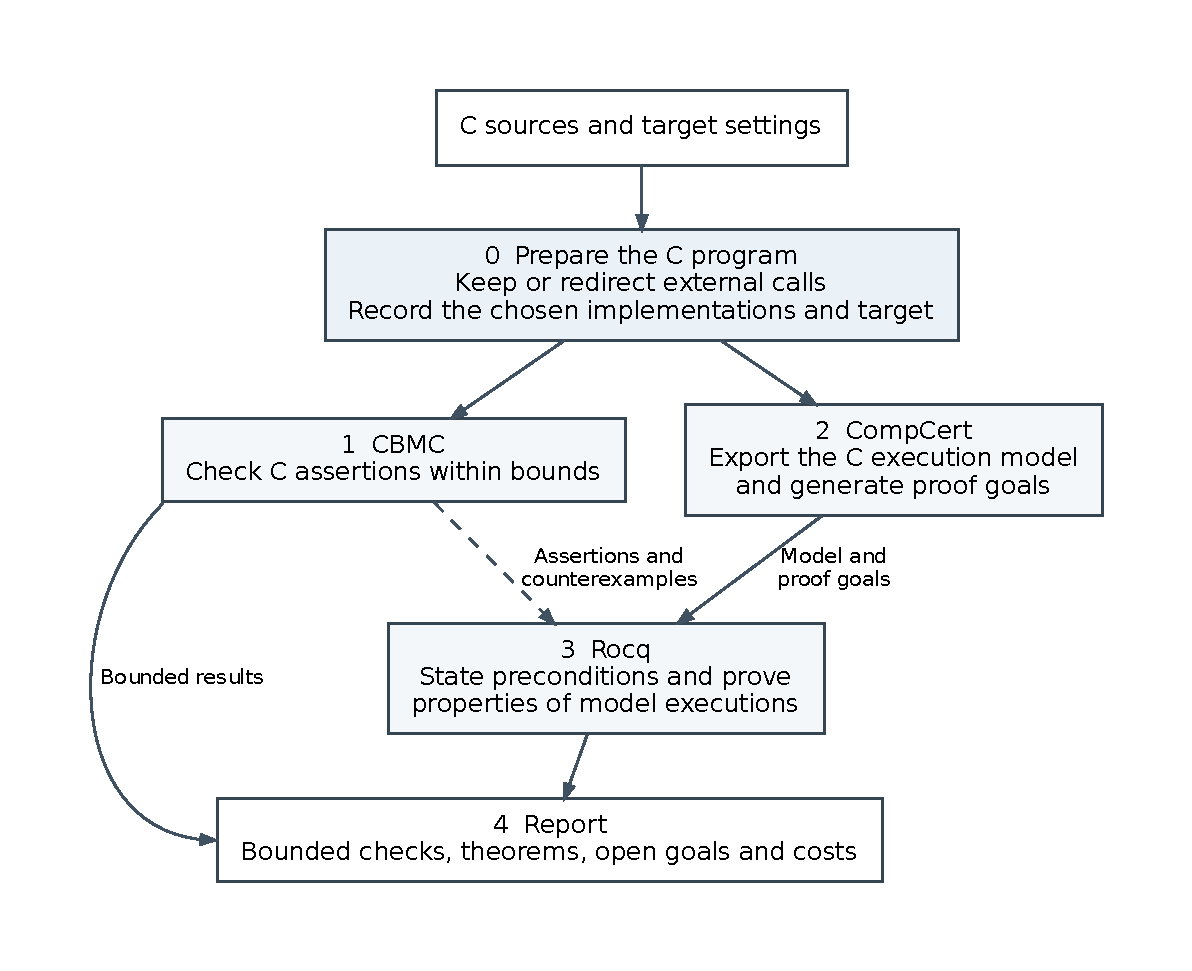
\includegraphics[width=\linewidth]{figures/five-framework.pdf}
  \caption{FIVE verification framework. Solid arrows carry artifacts;
  the dashed arrow supplies optional CBMC properties and counterexamples
  for independent analysis. Model generation creates pending goals, not
  completed proofs. Bounded CBMC evidence and Rocq theorems retain their
  respective scopes in the final report.}
  \Description{A common C source and semantic configuration feed CBMC
  bounded checking and CompCert model generation. Both supply artifacts
  to Rocq proof construction. CBMC evidence and checked Rocq theorems
  are collected with assumptions and costs in a scoped report.}
  \label{fig:five-framework}
\end{figure}

The three stages correspond to \texttt{five-cbmc}, \texttt{five-align},
and \texttt{five-rocq}. The wrapper \texttt{five-verify} coordinates their
handoffs and accounts for the evidence and resources of these stages. A model-generation request stops at pending goals, while
a proof request supplies preconditions and proof terms. Rocq can also
accept existing models independently of CBMC. This separation makes an
unfinished proof visible instead of treating model export as verification.

\subsection{Verification objective and semantic baseline}

The objective is to prove functional properties of a floating-point C
program while retaining the effects of finite-precision evaluation. A real
arithmetic recurrence is not, in general, a sufficient specification of a
floating-point filter. Consider the Paparazzi second-order low-pass filter
used in our aviation case. Its C implementation computes
\[
 y = b_0 x + b_1 i_0 + b_0 i_1 - a_0 o_0 - a_1 o_1,
\]
where $i_0,i_1$ and $o_0,o_1$ are the stored input and output histories.
Writing this recurrence over real numbers hides the rounding performed by
each multiplication and by the left-associated additions and subtractions.
If $\operatorname{fl}_{32}$ denotes rounding to the selected binary32
format, the corresponding computational structure is
\[
\begin{aligned}
 r_0 &= \operatorname{fl}_{32}(b_0 x),\\
 r_1 &= \operatorname{fl}_{32}(r_0+\operatorname{fl}_{32}(b_1 i_0)),\\
 r_2 &= \operatorname{fl}_{32}(r_1+\operatorname{fl}_{32}(b_0 i_1)),\\
 r_3 &= \operatorname{fl}_{32}(r_2-\operatorname{fl}_{32}(a_0 o_0)),\\
 y   &= \operatorname{fl}_{32}(r_3-\operatorname{fl}_{32}(a_1 o_1)).
\end{aligned}
\]
These equations illustrate the rounding structure for finite operands;
the actual model uses CompCert floating-point operations, including its
exceptional-value semantics. Reassociating the terms or using a fused
operation can change the output bits. The function then shifts both
histories, stores the current input and output, and returns the output.
Consequently, an exact functional specification must also account for the
updated memory bytes. A different computational structure requires a
separate bitwise-equivalence argument, rather than an appeal to algebraic
equality over the reals.

The current artifacts use CompCert 3.17 on x86-64 Linux, with little-endian
memory, binary32 operations, round-to-nearest ties-to-even and the pinned
CompCert NaN policy. Our semantic baseline fixes the CompCert version and target configuration
used for each experiment, including architecture, ABI, endianness, floating
formats, rounding, and the treatment of exceptional floating-point values.
The C translation is obtained from the source with CompCert's C front end;
the execution model uses the original CompCert C semantics and executable
semantics. The resulting model directly reuses CompCert's C execution definitions. CompCert connects these source semantics to target execution through its
compiler-correctness theorem for defined source behaviors. Fixing the
architecture, floating-point environment and external interfaces therefore
provides a common basis for both formal reasoning and compiled execution
\cite{Leroy2009}. Appendix~\ref{app:sum3-baseline} runs CompCert-generated
x86-64 code and checks its returned bits against the Rocq computation,
including a NaN payload example.

The model admits the program's machine-level inputs without imposing a
numeric filter such as finiteness or non-NaN values. A theorem may state
preconditions required by a caller, data structure, or safety property, but
those assumptions are recorded with that theorem and are not silently
folded into the execution model. The verification target includes observable
floating-point results and, when the program uses casts, unions, byte
operations, or pointer reinterpretation, the relation between values and
the bytes read or written in C memory. IEEE-style floating-point theories
make the operation semantics explicit, but a value-level result alone does
not establish a byte-level memory property \cite{Brain2015}.

\subsection{Why verification is divided into levels}

The central design choice is to separate implementation checks, semantic
anchoring, and functional reasoning. Each task contributes its own evidence through the corresponding proof mechanism. Bit-precise bounded model checking is useful for finding concrete
violations and checking local C properties, but its completeness depends on
the unwinding bounds. A source-level proof can establish an inductive
property for every reachable state, but only if the formal model is tied to
the program and the property accurately describes the required behavior.
An executable model can expose rounding and memory effects, but execution
examples alone do not prove a universal theorem.

This separation is especially relevant to floating-point code. Precise
floating-point theories are available to automated reasoning tools; their
existence does not imply that a solver will discharge every verification
condition produced by a large program. In practice, a condition can combine
rounding-sensitive arithmetic with path conditions, array indices, and
memory updates. The relevant automation cost therefore has to be measured
on the target programs. For CBMC, the evaluation protocol requires verification
outcomes together with unwinding bounds, time, and peak memory; a timeout or
out-of-memory result is not reported as a proof. Frama-C/WP documents both
the precise floating-point model and the fact that such obligations provide
limited support for automatic provers. Its Bytes memory model also
describes floating-point value-to-integer encoding through a conversion
function that the model assumes rather than defines. These properties determine the additional modeling and proof work
required for our bit-level observations \cite{FramaCWPManual}.

The required specification also spans different abstraction levels.
Contracts and separation-logic assertions are useful for describing
function boundaries and memory footprints. For this work, however, the
high-level properties include relationships across multiple calls and
control cycles. They are naturally expressed with recursive definitions,
inductive predicates, and lemmas in a proof assistant. CBMC's ordinary
bounded workflow can establish a property up to a chosen loop-unwinding
bound; this alone does not imply the property for an arbitrary number of
cycles \cite{KroeningTautschnig2014}. An inductive invariant or a proof that
the bound covers every execution is still required.

Table~\ref{tab:verification-levels} summarizes how the workflow assigns
these obligations. The workflow uses CBMC for direct, bit-precise analysis of
the C implementation, CompCert for the semantic account of the source, and
Rocq for properties whose proof requires induction or reusable functional
abstractions.

\begin{table*}[t]
\caption{Verification levels and the evidence each level contributes.}
\label{tab:verification-levels}
\centering
\begin{tabular}{@{}p{0.16\textwidth}p{0.20\textwidth}p{0.29\textwidth}p{0.25\textwidth}@{}}
\hline
Level & Main mechanism & Suitable obligations & Scope of the result \\
\hline
Implementation & Traditional CBMC bounded model checking & Array and pointer safety, conversions and bit operations, and local assertions over the original C & Complete only for the stated bound or a separately justified complete unwind \\
Model generation & CompCert C front end and original Csem/Cexec semantics & Exported syntax, provenance, pending goals and mapped property statements & Source-bound artifacts; correspondence and program goals remain proof obligations \\
Proof construction & Rocq definitions, lemmas, and induction & Correspondence, CBMC-property reproof, safety, termination and functional invariants & Only completed theorems, under their stated preconditions and environment assumptions \\
\hline
\end{tabular}
\end{table*}

\subsection{Level 1: bounded checks of the C implementation}

At the first level, CBMC analyzes the selected original C source and its
verification entry points using its traditional symbolic-execution and
bounded-model-checking workflow. The harness states the input conditions
and properties for that verification case; the assertions remain
implementation-level C properties. Depending on the selected program and bound, they cover
array-index validity, pointer reads and writes, input constraints, bit
operations, data conversions, and local functional conditions. CBMC's
bit-precise encoding makes it suitable for examining finite-width
operations and supported floating-point constructs directly in C
\cite{KroeningTautschnig2014}.

Each result records the source revision, compiler and CBMC options,
preconditions, loop-unwinding bounds, assertions, solver result, wall-clock
time, and peak memory. A counterexample is retained with its path, input bit patterns and relevant
memory effects for comparison with the CompCert model. Reproduction may
use a semantic derivation in Rocq; fast direct interpreter evaluation is
not required and is not assumed to be available for every model. A successful bounded check is reported as
bounded unless the selected unwind is proved to cover every relevant
execution. This distinction prevents a finite exploration from being
presented as an unbounded safety theorem.

This level produces direct evidence about concrete C operations and
memory accesses, and discovers small counterexamples early. The observed
solver cost is an empirical result: the paper reports it per target and
property instead of inferring that a floating-point theory is inherently
intractable.

\subsection{Level 2: CompCert model and obligation generation}

The second level anchors each selected verification input to a formal C
execution model. CompCert's front end automatically translates the C
translation unit and its dependencies into its C abstract syntax. Rocq then
uses the original CompCert C execution semantics rather than a manually
implemented interpreter. This gives the proof a machine-checked account of
C expressions, control flow, calls, and memory under a fixed CompCert
version and target configuration \cite{Leroy2009,Ramananandro2016}.

The alignment check binds the generated syntax tree and executable model
to the selected C files, headers, preprocessing options, and target
metadata. Regeneration is compared with the committed model so that a
stale or hand-edited export cannot silently become the proof input. The preprocessing and front-end export chain, together with the chosen
external contracts, form the explicitly recorded trust boundary. Model
state includes the CompCert memory state. Where a property observes memory
as bytes, the proof states the representation relation between a C
floating-point value, its bit pattern, and the affected byte range; a
value-level floating-point theorem is not used as a substitute for this
relation.

CBMC results are not imported into Rocq as axioms or trusted certificates.
For each selected assertion, this stage records the corresponding proposition
as a pending task over the CompCert execution model. The subsequent Rocq
proof stage must establish or refute it independently. The reproof uses the
same C source, precondition, program point, observable result, and stated
bound. If the Rocq theorem proves a stronger
unbounded statement, that stronger scope is reported explicitly. A
mismatch can reveal an extraction, configuration, or specification error;
agreement supplies proof-backed evidence for the selected property under
the formal C semantics.

CompCert export binds each formal execution model to its selected C input.


\subsection{Explicit safety and termination obligations}

The execution domain is separate from the proof precondition. Let
$\operatorname{entry}_f(a,m)$ be a function-call state for argument values
$a$ and CompCert memory $m$, and let $s\longrightarrow s'$ mean that a
Csem transition exists with some trace. The selected function-level error
predicate is
\[
 \operatorname{Error}(s) \equiv
 \neg\operatorname{NormalReturn}(s)\ \land\
 \neg\exists s'.\;s\longrightarrow s'.
\]
Here a normal return has the designated function boundary's stop
continuation. This is a semantic no-progress condition, not a claim that
the host operating system produces a crash. NaN and infinity are values,
not errors by this definition. Exhausting interpreter fuel also does not
establish an error. Missing external-call support must be resolved against
an explicit environment contract before it is interpreted as program failure.

For every new export, the generator produces separate precondition,
obligation and proof-template files. With a still-unspecified predicate
$P(a,m)$, the safety target is
\[
 \forall a,m,s.\quad P(a,m)\land
 \operatorname{entry}_f(a,m)\longrightarrow^{*}s
 \ \Rightarrow\ \neg\operatorname{Error}(s).
\]
The termination target requires accessibility of the successor relation
from the entry state, with relation orientation
$R(s',s)\equiv s\longrightarrow s'$. Thus every execution branch must be
well founded, rather than just one selected evaluation path terminating.
Safety and termination are independent obligations: a stuck state can be
well founded, and an infinite execution can have progress at every step.
Together they exclude both stuck maximal executions and infinite ones,
under the stated transition semantics and precondition.

The generator does not select a convenient input domain or insert an
assumed theorem. During proof construction, the author supplies $P$, checks
that it captures the caller contract and has meaningful inhabitants, and
proves the requested goals. A typical safety argument establishes an
invariant at entry, proves preservation by every transition, and derives
progress or normal return at every reachable state. Induction over
reachability then establishes the target without enumerating paths.
Termination additionally needs a well-founded argument; the invariant
alone does not imply it. The historical cases retain different proof
organizations and are not all complete instances of the new generator.

\subsection{Level 3: proof construction and functional properties in Rocq}

At the third level, Rocq proves properties that are awkward to express as
bounded assertions over a single C execution. The functional specification
is an executable or inductive model whose operations preserve the
target-relevant floating-point evaluation order. It may expose a more
abstract state than the C heap, but the abstraction is accompanied by an
explicit relation to the CompCert state and memory. No alternative
real-number expression is assumed to be bitwise equivalent merely because
it is algebraically equal.

Proofs are organized compositionally. First, function-level theorems state
the transitions and memory effects of individual operations. Next, these
theorems are composed to establish a control-cycle property. Finally, an
induction over the cycle count proves the desired property for every finite
execution length. The induction invariant is written as a Rocq predicate
over reachable states; the proof establishes that the initial state
satisfies it and that every semantic transition preserves it. This provides
an unbounded argument without enumerating paths or selecting a finite
number of cycles.

The model exposes the full execution domain. Theorem preconditions
describe the caller requirements, such as a valid caller-owned object
or an initialized state required by a function contract. NaNs, infinities, signed zero, subnormal values, and overflow are
handled according to the pinned formal semantics wherever that semantics
defines the operation. Any additional assumptions needed for a particular
functional claim are stated next to the claim.

\subsection{Why CompCert and Rocq form the proof backbone}

The method chooses CompCert and Rocq because the main assurance gap is the
connection from a concrete C execution to an inductive functional theorem.
CompCert supplies the generated source representation and C execution
semantics used in that connection. Rocq supports the definitions and
inductive proofs needed for high-level behavior, while retaining kernel
checking of the completed terms. CBMC complements these components by
checking bounded, implementation-specific obligations with little model
construction overhead.

Each stage attaches its conditions to its result: CBMC records the checked
bound, model generation records the C source and target configuration, and
Rocq records the quantified precondition and proved statement. The CompCert
compiler connects defined source behavior to its target implementation.
Rounding, representation and memory lemmas then support reusable functional
proofs over this common execution foundation.

Three alternatives clarify the choice. Using CBMC alone retains direct C
analysis, but ordinary finite unwinding does not supply an arbitrary-cycle
induction proof. Using only a hand-translated Rocq model makes high-level
reasoning convenient, but adds a separate translation-correctness problem
for every program, including its error and memory behavior. Generating the
syntax with CompCert and reusing Csem/Cexec avoids maintaining a second,
program-specific implementation of C execution. It does not eliminate
source-export provenance checks, external-environment assumptions, or
proofs relating any higher-level abstraction to that execution.

Rocq is selected here because CompCert's semantic definitions and supporting
proofs are already available in the same logic. This permits direct reuse
of its memory and floating-point infrastructure without introducing another
cross-assistant semantic translation. Direct reuse of these definitions simplifies integration. Interactive
proof construction contributes its own token, time and memory costs,
which are measured alongside the automated checks.

For exact functional specifications, a contract still needs a definition
of the required computation. For example, specifying the low-pass filter solely by its real-valued
recurrence omits the rounding at each product and accumulation, as well
as the precise history updates. A contract may instead refer to the
ordered floating-point computation and its memory effects. Choosing
a contract framework therefore changes how the proof is organized, but
does not in itself remove the need for a precise functional model and its
connection to the implementation. Reusable high-level properties are stated
separately from this model, so that correctness is not reduced to restating
the execution definition.

\begin{sloppypar}
The framework selection follows three concrete requirements: preservation
of rounded floating-point operations, explicit correspondence with stored
bits and bytes, and reusable proofs over all reachable states. CompCert
provides the execution and representation definitions, and Rocq provides
the logic in which those definitions and inductive proofs are maintained.
CBMC supplies bounded implementation checks and concrete counterexamples.

The comparison with contract-driven frameworks is grounded in the
experiments in Appendices~\ref{app:sum3-baseline} and~\ref{app:wp-bytes}.
QCP v2.1.4 preserves the two rounded additions in sum3 but uses a NaN
callback whose output bits differ from the selected CompCert x86-64
policy and the measured native results. Adopting that release therefore
requires a matching NaN policy and its correspondence proof. For
Frama-C/WP, the decisive issue is the value-to-byte connection: the tested
Bytes model exposes an abstract floating-point encoding interface instead
of the concrete IEEE binary32 codec. Even the byte representation of
\texttt{1.0f} consequently requires additional encoding definitions and
proof support. The official WP manual documents this modeling choice
\cite{FramaCWPManual,QCPFloatLib214}.

FIVE selects CompCert and Rocq to reuse one concrete execution and memory
foundation across arithmetic, representation and functional reasoning.
The choice follows the required semantic coverage and integration work.
The Unresolved WP arithmetic goals characterize the tested prover configurations;
the stronger selection evidence is the inspected encoding interface and
the measured QCP NaN-policy difference. The generated obligations and
their proof status remain explicit artifacts of each verification task.
\end{sloppypar}

\subsection{Counterexample-guided refinement and evidence}

The levels form a feedback process. A CBMC counterexample is checked against its harness and mapped to a
CompCert execution under matching inputs, memory and observations. The
model-side reproduction is established by execution or a semantic proof;
a missing reproduction is reported as pending. If the two differ, the source model,
target configuration, or property encoding is investigated before the
functional theorem is trusted. If they agree and expose a defect, the
implementation or its stated precondition is corrected. If a Rocq proof
fails, the resulting unsolved obligation is used to refine the invariant,
supporting lemma, or specification; it is not discharged by weakening the
claim without recording the change.

The reporting protocol requires, for each case, the C and generated-model hashes, the
CompCert configuration, the CBMC properties and bounds, the Rocq theorem
statements and assumptions, and actual input/output tokens, wall time, tool CPU time and observed peak
process memory. Failed attempts remain in the record; missing measurements
are marked incomplete, and shared events are deduplicated rather than
charged repeatedly. Repository editing and paper compilation are not
verification-stage measurements. An end-to-end claim
is made only when the relevant implementation checks, independent property
proofs, and semantic correspondence obligations agree. Tests and bounded
checks remain useful evidence, while an arbitrary-cycle functional claim
rests on the Rocq induction and its proved link to CompCert execution.

\section{Empirical Evaluation}


Here we focus on real-world application and engineering value rather than standard benchmark metrics. 
\subsection{Experimental Setup and Case Description}

Yang Fanpeng: Introduce the real-world aerospace software assets (e.g., satellite sun-search control system or flight control software).
\subsection{RQ1: Effectiveness of Entity and Interface Extraction}


Ma Xu 
\subsection{RQ2: Verification Effectiveness and Cost}

RQ2 asks which obligations are discharged at each level and what resources
the verification requires on the selected aerospace programs. For every
CBMC property, we record its source location, precondition, unwind bound,
result (proved within bound, counterexample, timeout, or resource failure),
wall-clock time, and peak memory under a fixed tool configuration. We report
the number of discharged properties divided by the number attempted, while
listing timeouts and incomplete unwinds separately; neither is counted as a
proof. These measurements provide the evidence for claims about CBMC's
automation cost on these programs.

For the CompCert and Rocq levels, the evaluation protocol records verification-source hashes,
target metadata, regeneration and semantic-alignment results, theorem
statements, assumptions, kernel-check status, input/output token usage,
wall time, tool CPU time and observed peak memory. A generated obligation
is recorded separately from a completed proof. Cached input and reasoning
output are subsets of their respective token totals, not additional charges.
The extraction/interface cases from RQ1 and the verification cases from RQ2
are reported as separate populations.
We classify properties by implementation safety, local functional behavior,
memory-byte correspondence, cross-function behavior, and cycle invariants.
This makes it possible to see which obligations require each level and
whether any claim depends on a narrower input domain or a finite bound.

No aggregate success rate or resource figure is inferred from a subset of
cases. Appendix~\ref{app:sum3-baseline} provides an executed comparison of
rounding, NaN representation and native output bits. The remaining
aerospace-case measurements will populate the broader RQ2 evaluation.
 \subsection{Others??}
 

\section{Related Work}

\section{Discussion and Lessons Learned}

\section{Conclusion}

\bibliographystyle{ACM-Reference-Format}
\bibliography{references}


\clearpage
\appendix
\section{Sum3: Measured Agreement with Native Execution}
\label{app:sum3-baseline}

This experiment connects CompCert's floating-point operations to actual
x86-64 execution and compares the arithmetic models used by WP and QCP.
The aviation low-pass filter remains the main example; the following
straight-line function isolates rounding and NaN representation:

\begin{verbatim}
float sum3(float a, float b, float c) {
    return a + b + c;
}
\end{verbatim}

\subsection{Experimental configuration and procedure}

We ran the experiment on November 3, 2026, using x86-64 Linux under WSL2,
CompCert 3.17, GCC 11.4.0, Rocq 9.2, Frama-C/WP 31.0 (Gallium), and the
original QCP v2.1.4 release binary. The target uses little-endian binary32
and nearest-even rounding. The native harness sets MXCSR to
\texttt{0x1f80}: exceptions are masked and gradual underflow is enabled.
Inputs are supplied as exact 32-bit words through \texttt{memcpy}.

CompCert compiles \texttt{sum3} as a separate translation unit. Its object
code contains two successive \texttt{addss} instructions and is linked to
the bit-pattern harness. A GCC build provides a second native comparison,
using \texttt{-O0}, \texttt{-fno-fast-math}, \texttt{-ffp-contract=off},
and \texttt{-frounding-math}. Both executables print the returned word.
In Rocq, we evaluate the corresponding two \texttt{Float32.add}
operations and independently kernel-check the result-bit theorems.

QCP is actually run with \texttt{--arch=64}, \texttt{--endian=little},
and \texttt{--no-float-finite-vc}. Its symbolic execution produces
\texttt{fp32\_add (fp32\_add a b) c}. We compile the unchanged release
\texttt{FloatLib.v} in the same Rocq environment and kernel-check the two
result-bit theorems for this expression. The QCP contract uses
\texttt{Require emp / Ensure emp}, leaving the input values unrestricted;
bit equality is checked by the Rocq theorems rather than IEEE equality.
Thus the measured proof artifacts are the four arithmetic result-bit
theorems, alongside QCP's recorded symbolic execution.

WP is run twice on identical contracts, with \texttt{Typed+real} and
\texttt{Typed+float}, the x86-64 machine model, and Qed. For the finite
input below, separate postconditions ask whether the result equals zero
or one. The archive records the complete commands, outputs, tool and
source hashes, proof assumptions, and cost receipts in
\path{paper/experiments/sum3/}.

\subsection{Rounding and native agreement}

The first input is $a=2^{24}$, $b=1$, $c=-2^{24}$, represented by
\texttt{0x4b800000}, \texttt{0x3f800000}, and \texttt{0xcb800000}.
Nearest-even rounding gives
\[
 \operatorname{fl}_{32}(\operatorname{fl}_{32}(2^{24}+1)-2^{24})=+0.
\]
Both native executables return \texttt{0x00000000}, exactly matching the
CompCert theorem. QCP's library expression also returns that word.

For WP's Real model, the zero-result verification condition reduces to
\texttt{false}, while Qed proves the one-result postcondition. Its
abstraction computes the real-valued sum, which is $1$. For WP's Float
model, the printed condition retains
\texttt{add\_f32(add\_f32(a,b),c)}; Qed reports \emph{Unknown} for both
postconditions. These observed outcomes separate a rounding abstraction
from an automatic-proof limitation. WP uses weakest-precondition
generation, while QCP uses separation-logic symbolic execution
\cite{FramaCWPManual,WuEtAl2026}.

\subsection{NaN payloads and bit-level agreement}

The second input uses words \texttt{0x7fc00042}, \texttt{0x00000000},
and \texttt{0x00000000}. The first operand is a quiet NaN with a
nondefault payload. Table~\ref{tab:sum3-measured} reports the actual
returned words and the kernel-checked arithmetic results.

\begin{table}[h]
\centering
\caption{Measured return words for the two sum3 inputs.}
\label{tab:sum3-measured}
\begin{tabular}{lll}
\hline
Execution or model & Finite input & NaN input \\
\hline
CompCert operations in Rocq & \texttt{00000000} & \texttt{7fc00042} \\
CompCert-compiled native code & \texttt{00000000} & \texttt{7fc00042} \\
GCC-compiled native code & \texttt{00000000} & \texttt{7fc00042} \\
QCP library expression in Rocq & \texttt{00000000} & \texttt{7f800001} \\
\hline
\end{tabular}
\end{table}

CompCert's x86-64 policy selects the first NaN operand and quiets its
payload. Here that operand is already quiet, so both additions preserve
\texttt{0x7fc00042}. Actual execution of the CompCert-generated instructions
preserves exactly those bits. QCP's inspected callback instead returns a
fixed positive NaN with payload $1$, giving \texttt{0x7f800001}; its
nearest-even rounding mode agrees with CompCert on the finite example
\cite{QCPFloatLib214,CompCertFloats317,CompCertArchi317}.

\subsection{Why FIVE uses CompCert as its execution baseline}

CompCert supplies both the formal C operations used in Rocq and a verified
compiler connecting defined source executions to generated target code
\cite{Leroy2009}. This shared semantic foundation supports bit-precise
floating-point verification. In this experiment, agreement with actual
execution includes the complete NaN encoding, rather than merely its
classification as NaN. The comparison is fixed to the versions, platform,
environment and two inputs specified above.

The experiment identifies the work needed to adopt the alternatives.
WP's Real abstraction removes rounding and therefore fails the finite
example. WP's Float model preserves the arithmetic structure, but Qed
does not discharge the tested result obligations. The independent byte-reading experiment in
Appendix~
ef{app:wp-bytes} identifies the concrete encoding relation
needed by WP's Bytes model. QCP performs the symbolic execution,
but its release NaN callback needs adaptation to match the chosen x86-64
bit semantics. FIVE directly reuses CompCert's operations, NaN policy and
memory model, then organizes the functional proofs in Rocq.

The measured experiment stage took 528.85 seconds wall time and 29.35
seconds tool CPU time. The observed tool-process-tree peak was
1,351,790,592 bytes. Session usage was 2,354,770 input tokens and 11,056
output tokens; 2,337,152 input tokens were cached. Two native processes
completed between the 10 ms memory samples, so the per-command sampling
audit records those entries as incomplete. The archive retains all runs,
including the initial contract attempt and its correction.


\clearpage
\section{Frama-C/WP: Floating-Point Values and Memory Bytes}
\label{app:wp-bytes}

This experiment directly tests the representation requirement used in
FIVE's framework selection. It asks whether reading the four bytes of
\texttt{1.0f} produces its binary32 encoding, \texttt{0x3f800000}, under
the fixed little-endian target. The example has no loop, arithmetic
rounding chain, NaN input, or external library call. Access through
\texttt{unsigned char} observes the C object's representation.

\begin{verbatim}
/*@ assigns \nothing;
    ensures \result == 0x3f800000; */
unsigned int bits_one(void) {
  float x = 1.0f;
  const unsigned char *p = (const unsigned char *)&x;
  return (unsigned int)p[0]
       | ((unsigned int)p[1] << 8)
       | ((unsigned int)p[2] << 16)
       | ((unsigned int)p[3] << 24);
}
\end{verbatim}

\subsection{Executed configurations and results}

We ran Frama-C/WP 31.0 (Gallium) with \texttt{-machdep x86\_64},
runtime-error obligations enabled, and two memory configurations:
\texttt{Typed+float} and \texttt{Bytes+raw+float}. The latter activates
the byte model throughout the function. Qed was used first, followed by
Alt-Ergo 2.6.2 and Z3 4.13.3 with a five-second limit per attempt for the
Bytes configuration. GCC 11.4 and CompCert 3.17 compiled the same function
for native execution; both executables returned \texttt{0x3f800000}.

The Typed configuration reported a pointer-cast modeling
warning for the float-to-character pointer cast. The Bytes configuration
generated the byte-access obligations. Alt-Ergo and Z3 each proved all
four read-validity obligations and the \texttt{assigns} obligation. Both
timed out on the remaining postcondition fixing the returned encoding.
The successful memory-safety obligations isolate the unresolved property:
the connection between the stored floating-point value and its exact bytes.

\subsection{Inspecting the generated encoding interface}

The exported solver input contains abstract encoding and decoding
functions, together with inverse axioms. In schematic notation, their
interface is:
\[
 \operatorname{encode}:\operatorname{Float32}\to\mathbb{Z},\qquad
 \operatorname{decode}:\mathbb{Z}\to\operatorname{Float32}.
\]
WP names these functions \texttt{float32\_to\_int} and
\texttt{int\_to\_float32}. The initializer contributes the constraint
\[
 \operatorname{decode}(\operatorname{read32}(m,\operatorname{addr}(x)))
   = \operatorname{to\_f32}(1.0).
\]
The postcondition requires the concrete word $1065353216$, namely
\texttt{0x3f800000}. The interface does not specify the IEEE encoding
equation
\[
 \operatorname{encode}(\operatorname{to\_f32}(1.0))=1065353216.
\]
Thus the source of the integration work is visible in the actual generated
model, beyond the observed solver timeout. The WP 33.0 manual, Section~3.8,
independently documents that the Bytes model assumes a floating-point
conversion function without giving its concrete definition
\cite{FramaCWPManual}.

\subsection{Consequence for bit-precise verification}

For FIVE, floating-point results and their stored representations are part
of the same verification target. Using WP for this target requires a
concrete encoding model and supporting correspondence lemmas. CompCert
already provides concrete floating-point bit conversions and memory
encoding definitions in the semantic infrastructure reused by Rocq.
This is the basis for our choice: it keeps arithmetic, NaN handling and
byte-level observations within one target-specific execution semantics.

The executed configurations, complete solver inputs, native outputs,
source hashes and cost records are available in
\path{paper/experiments/float-bytes/}. The distinction is precise: the
observed postcondition outcome is a timeout, while the documented and
inspected modeling issue is the abstract encoding interface. The native
comparison in this experiment establishes the observed word; the separate
sum3 experiment also supplies kernel-checked arithmetic result-bit theorems.

\end{document}
\endinput
%%
%% End of file `acmsmall-submission.tex'.
